% !TeX root = booklet-02.tex
\subsection{اثرهای ولتاژ آستانه}
\label{sec:threshold-effects}
ولتاژ آستانه، مقدار ولتاژ \lr{Gate} نسبت به \lr{Source} برای آغاز وارونگی
در مدل است. در تقریب‌های قبلی آن را ثابت گرفتیم. اکنون تغییر آن با بایاس
بدنه، بایاس درین و طول کانال را بررسی می‌کنیم
\cite[بخش \secnum{۲.۴.۳}]{weste}\cite[اسلاید ۱۵]{nonideal}.
هنگام تغییر آستانه، اضافه‌ولتاژ گیت \(V_{GT}=V_{GS}-V_t\) نیز باید
دوباره محاسبه شود. مثبت‌بودن اضافه‌ولتاژ و شرط ناحیه کاری، پس از این
به‌روزرسانی کنترل می‌شوند.

\subsubsection{\lr{Body Effect}}
\label{sec:body-effect}
\paragraph*{بدنه، پیوند معکوس و بار لازم برای وارونگی}
در \lr{Bulk nMOS}، بدنه \lr{p-type} و ناحیه‌های \lr{Source} و
\lr{Drain} از نوع \lr{n-type} هستند. ولتاژ بدنه را \(V_B\) می‌نامیم.
بایاس سورس نسبت به بدنه برابر \(V_{SB}=V_S-V_B\) است. در شرایط
\(V_{SB}\ge0\)، پیوند سورس و بدنه در بایاس صفر یا معکوس قرار دارد.
افزایش بایاس معکوس، بار تخلیه‌ای را که گیت باید برای رسیدن به وارونگی
جبران کند افزایش می‌دهد. به همین علت، آستانه افزایش می‌یابد
\cite[بخش \secnum{۲.۴.۳.۱}]{weste}\cite[اسلاید ۱۶]{nonideal}.

اگر \(V_S=\qty{0.6}{\volt}\) و \(V_B=0\) باشند،
\(V_{SB}=\qty{0.6}{\volt}\) است. اگر همین دو پایانه در
\(\qty{0.6}{\volt}\) به هم متصل شوند، \(V_{SB}=0\) می‌شود.
اختلاف ولتاژ سورس و بدنه، کمیت ورودی رابطه اثر بدنه است.

\paragraph*{رابطه کامل آستانه و معنای نمادها}
کتاب و اسلاید ۱۶ رابطه زیر را برای اثر بدنه معرفی می‌کنند
\begin{equation}
 \boxed{V_t=V_{t0}+\gamma
 \left(\sqrt{\phi_s+V_{SB}}-\sqrt{\phi_s}\right)}.
 \label{eq:threshold-body}
\end{equation}
در این رابطه، \(V_{t0}\) آستانه در بایاس صفر سورس و بدنه،
\(\phi_s>0\) پتانسیل سطحی در آستانه و \(\gamma>0\) ضریب اثر بدنه
است \cite[رابطه \secnum{۲.۳۵}]{weste}. \(\phi_s\)، \(V_{t0}\) و
\(\gamma\) برای شرایط فناوری و دمای معین تعریف می‌شوند.
در این قسمت، تغییر بایاس بدنه را با ثابت گرفتن آن پارامترها تحلیل می‌کنیم.
اثر بایاس درین در بخش \ref{sec:dibl-effect} وارد می‌شود.

عملگر \(\sqrt{a}\)، ریشه مثبت عدد نامنفی \(a\) است. برای مثال،
\(\sqrt{0.81}=0.9\)، زیرا \((0.9)^2=0.81\).
در \eqref{eq:threshold-body}، هر عبارت زیر رادیکال واحد ولت دارد، پس
ریشه آن واحد \(\mathrm{V}^{1/2}\) دارد. برای ولتاژ شدن حاصل‌ضرب، واحد
\(\gamma\) نیز باید \(\mathrm{V}^{1/2}\) باشد.

در بایاس صفر، دو ریشه برابر و \(V_t=V_{t0}\) است. برای
\(V_{SB}>0\)، ریشه اول بزرگ‌تر می‌شود، بنابراین \(V_t>V_{t0}\).
در تحلیل این جزوه، دامنه معمول بایاس معکوس \(V_{SB}\ge0\) را به کار
می‌بریم. انتخاب بایاس عملی به شرایط مجاز پیوندها و پارامترهای فرایند
وابسته است.

\paragraph*{غلظت ناخالصی، ولتاژ حرارتی و پتانسیل سطحی}
کتاب پتانسیل سطحی را با غلظت ناخالصی پذیرنده \(N_A\)، غلظت ذاتی
حامل‌ها \(n_i\) و ولتاژ حرارتی \(v_T\) مرتبط می‌کند
\begin{equation}
 \phi_s=2v_T\ln\!\left(\frac{N_A}{n_i}\right),\qquad
 v_T=\frac{kT}{q}.
 \label{eq:threshold-surface-potential}
\end{equation}
در اینجا \(T\) دمای مطلق برحسب کلوین، \(k\) ثابت \lr{Boltzmann} و
\(q>0\) بزرگی بار الکترون است
\cite[رابطه \secnum{۲.۳۶} و مثال \secnum{۲.۵}]{weste}.
نماد کوچک \(v_T\) برای ولتاژ حرارتی و نماد \(V_t\) برای آستانه به کار
رفته است. در تقریب اتاق کتاب، \(T\approx\qty{300}{\kelvin}\) و
\(v_T\approx\qty{0.026}{\volt}\) هستند.

چون لگاریتم روی یک نسبت بی‌بعد اعمال می‌شود، \(N_A\) و \(n_i\) باید
با واحد یکسان نوشته شوند. برای مثال، اگر هر دو برحسب
\(\unit{\per\centi\metre\cubed}\) باشند، واحد در نسبت حذف می‌شود.
\(\ln\) همان لگاریتم طبیعی معرفی‌شده در مرور پیش‌نیاز است.
اگر \(N_A>n_i\) باشد، لگاریتم مثبت و \(\phi_s>0\) می‌شود.

برای تبدیل غلظت، چون \(\qty{1}{\centi\metre\cubed}
=\qty{e-6}{\metre\cubed}\)، داریم
\(\qty{2e17}{\per\centi\metre\cubed}
=\qty{2e23}{\per\metre\cubed}\).
استفاده از واحد سانتی‌متر در \(N_A\) و واحد متر در
\(\varepsilon_{\mathrm{si}}\) به تبدیل سازگار نیاز دارد.

\paragraph*{ضریب اثر بدنه و کنترل ابعاد}
دو شکل معادل ضریب اثر بدنه در مرجع چنین‌اند
\begin{equation}
 \gamma=\frac{\sqrt{2q\varepsilon_{\mathrm{si}}N_A}}{C_{\mathrm{ox}}}
 =\frac{t_{\mathrm{ox}}}{\varepsilon_{\mathrm{ox}}}
 \sqrt{2q\varepsilon_{\mathrm{si}}N_A}.
 \label{eq:threshold-gamma}
\end{equation}
در این رابطه، \(\varepsilon_{\mathrm{si}}\) و
\(\varepsilon_{\mathrm{ox}}\) به‌ترتیب \lr{Permittivity} سیلیکون و اکسید
هستند. برابری دو شکل از
\(C_{\mathrm{ox}}=\varepsilon_{\mathrm{ox}}/t_{\mathrm{ox}}\) به دست
می‌آید \cite[رابطه \secnum{۲.۳۷}]{weste}.
برای کنترل واحد، \(B_Q=\sqrt{2q\varepsilon_{\mathrm{si}}N_A}\) را
تعریف می‌کنیم. با \(\mathrm{F}=\mathrm{C}/\mathrm{V}\)، داریم
\begin{align}
 [B_Q]&=\sqrt{\mathrm{C}\,
 \frac{\mathrm{F}}{\mathrm{m}}\,
 \frac{1}{\mathrm{m}^3}}
 =\frac{\mathrm{C}}{\mathrm{m}^2\sqrt{\mathrm{V}}},\notag\\
 [\gamma]&=\frac{\mathrm{C}/(\mathrm{m}^2\sqrt{\mathrm{V}})}
 {\mathrm{F}/\mathrm{m}^2}=\sqrt{\mathrm{V}}.
 \label{eq:threshold-gamma-units}
\end{align}
این نتیجه با واحد لازم در \eqref{eq:threshold-body} سازگار است.
با ثابت بودن بقیه پارامترهای این مدل، افزایش ضخامت اکسید،
\(C_{\mathrm{ox}}\) را کم و \(\gamma\) را زیاد می‌کند.

\paragraph*{استخراج آموزشی رابطه از بار تخلیه}
برای توضیح منشأ رادیکال، تقریب تخلیه و ناخالصی یکنواخت را در نظر می‌گیریم.
بزرگی بار تخلیه بر واحد سطح را \(\sigma_{\mathrm{dep}}\) می‌نامیم.
بیان سازگار با مدل کتاب چنین است
\begin{equation}
 \sigma_{\mathrm{dep}}(V_{SB})
 =\sqrt{2q\varepsilon_{\mathrm{si}}N_A(\phi_s+V_{SB})}
 =B_Q\sqrt{\phi_s+V_{SB}}.
 \label{eq:threshold-depletion-charge}
\end{equation}
این رابطه، توضیح آموزشی مبنای \eqref{eq:threshold-gamma} و
\eqref{eq:threshold-body} است
\cite[بخش \secnum{۲.۴.۳.۱}، روابط \secnum{۲.۳۵} تا \secnum{۲.۳۷}]{weste}.
واحد \(\sigma_{\mathrm{dep}}\)، \(\unit{\coulomb\per\metre\squared}\)
است. در بایاس صفر، مقدار آن \(B_Q\sqrt{\phi_s}\) است.

تغییر ولتاژ لازم برای جبران بار اضافه روی ظرفیت اکسید از رابطه
\(\Delta V=\Delta\sigma/C_{\mathrm{ox}}\) به دست می‌آید.
بنابراین تغییر آستانه برابر است با
\begin{align*}
 \Delta V_t&=\frac{\sigma_{\mathrm{dep}}(V_{SB})-
 \sigma_{\mathrm{dep}}(0)}{C_{\mathrm{ox}}},\\
 &=\frac{B_Q}{C_{\mathrm{ox}}}
 \left(\sqrt{\phi_s+V_{SB}}-\sqrt{\phi_s}\right).
\end{align*}
با جایگذاری \(B_Q/C_{\mathrm{ox}}=\gamma\)، رابطه کامل اثر بدنه بازیابی
می‌شود. در این استخراج، افزایش بایاس بدنه از مسیر افزایش بار تخلیه به
افزایش آستانه مرتبط شده است.

\paragraph*{حل مثال \secnum{۲.۵} کتاب}
مثال مرجع، \(N_A=\qty{8e17}{\per\centi\metre\cubed}\)،
\(V_{t0}=\qty{0.3}{\volt}\) و اتصال بدنه به زمین را در نظر می‌گیرد.
سورس از صفر به \(\qty{0.6}{\volt}\) می‌رسد. در محاسبه ضریب بدنه در
ادامه حل کتاب، \(t_{\mathrm{ox}}=\qty{1.05}{\nano\metre}\) استفاده
شده است \cite[مثال \secnum{۲.۵} و رابطه \secnum{۲.۴۰}، صفحات ۷۹ و ۸۰]{weste}.
برای بازتولید نتیجه از ثابت‌های تقریبی همان کتاب استفاده می‌کنیم
\begin{align*}
 n_i&=\qty{1.45e10}{\per\centi\metre\cubed},
 &q&\approx\qty{1.6e-19}{\coulomb},\\
 \varepsilon_0&\approx\qty{8.85e-14}{\farad\per\centi\metre},
 &\varepsilon_{\mathrm{si}}&=11.7\varepsilon_0,
 &\varepsilon_{\mathrm{ox}}&=3.9\varepsilon_0.
\end{align*}
نماد \(\varepsilon_0\)، \lr{Permittivity} خلأ است. با
\(v_T\approx\qty{0.026}{\volt}\)، نسبت غلظت‌ها و پتانسیل سطحی چنین‌اند
\begin{align}
 \frac{N_A}{n_i}&=\frac{8\times10^{17}}{1.45\times10^{10}}
 \approx5.517\times10^7,\notag\\
 \phi_s&=2(0.026)\ln(5.517\times10^7)\,\unit{\volt}
 \approx\qty{0.92695}{\volt}.
 \label{eq:body-book-example-phi}
\end{align}
ضخامت اکسید در واحد سانتی‌متر،
\(\qty{1.05e-7}{\centi\metre}\) است. پس
\begin{align*}
 C_{\mathrm{ox}}&=\frac{3.9(8.85\times10^{-14})}{1.05\times10^{-7}}
 \approx\qty{3.2871e-6}{\farad\per\centi\metre\squared},\\
 B_Q&=\sqrt{2(1.6\times10^{-19})(11.7)(8.85\times10^{-14})(8\times10^{17})}
 \\
 &\approx\qty{5.1485e-7}{\coulomb\per\centi\metre\squared\per\volt\tothe{0.5}},\\
 \gamma&=\frac{B_Q}{C_{\mathrm{ox}}}
 \approx\qty{0.15663}{\volt\tothe{0.5}}.
\end{align*}
با \(V_{SB}=\qty{0.6}{\volt}\)، اکنون دو ریشه را جداگانه ارزیابی
می‌کنیم و تفاضل آن‌ها را در \(\gamma\) ضرب می‌کنیم
\begin{align*}
 \Delta V_t&\approx0.15663\left(\sqrt{0.92695+0.6}-\sqrt{0.92695}\right)
 \,\unit{\volt}\\
 &\approx\qty{0.04275}{\volt},\qquad
 V_t\approx\qty{0.34275}{\volt}.
\end{align*}
گردکردن به دقت متن مرجع، افزایش حدود \(\qty{0.04}{\volt}\) و آستانه
\(\qty{0.34}{\volt}\) را می‌دهد. رقم‌های بیشتر برای دنبال‌کردن محاسبه
میانی آورده شده‌اند. کتاب در توضیح عمومی \(\gamma\)، بازه معمول
\(\qty{0.4}{\volt\tothe{0.5}}\) تا
\(\qty{1}{\volt\tothe{0.5}}\) را ذکر می‌کند. محاسبه هر نمونه با
پارامترهای همان نمونه انجام می‌شود و در مثال حاضر، ضریب حدود
\(\qty{0.16}{\volt\tothe{0.5}}\) به دست آمده است.

\paragraph*{خطی‌سازی با استفاده از تفاضل دو مربع}
برای دیدن تقریب بایاس کوچک، \(U=V_{SB}\) می‌گذاریم. اتحاد
\((a-b)(a+b)=a^2-b^2\) برای دو ریشه می‌دهد
\begin{equation}
 \sqrt{\phi_s+U}-\sqrt{\phi_s}
 =\frac{U}{\sqrt{\phi_s+U}+\sqrt{\phi_s}}.
 \label{eq:body-rationalized-root}
\end{equation}
این تبدیل، دقیق است. اگر \(U\ll\phi_s\)، ریشه اول به
\(\sqrt{\phi_s}\) نزدیک است، پس مجموع دو ریشه را تقریباً
\(2\sqrt{\phi_s}\) می‌گیریم. ازاین‌رو
\begin{equation}
 \Delta V_t\approx\frac{\gamma U}{2\sqrt{\phi_s}}
 =k_\gamma U,\qquad
 k_\gamma=\frac{\gamma}{2\sqrt{\phi_s}}.
 \label{eq:body-linearization}
\end{equation}
این نتیجه با روابط \secnum{۲.۳۸} و \secnum{۲.۳۹} کتاب و اسلاید ۱۷
برابر است \cite{weste,nonideal}. واحد \(k_\gamma\) بی‌بعد است.
شیب دقیق در بایاس \(U\) نیز از مشتق رادیکال به دست می‌آید
\begin{equation}
 \frac{\mathrm{d}V_t}{\mathrm{d}U}
 =\frac{\gamma}{2\sqrt{\phi_s+U}}.
 \label{eq:body-slope}
\end{equation}
در \(U=0\)، این شیب برابر \(k_\gamma\) است و با افزایش \(U\) کاهش
می‌یابد. آستانه همچنان افزایش می‌یابد، اما افزایش آن به ازای هر ولت
بایاس کمتر می‌شود.

با جایگذاری \(\gamma\) و \(\phi_s\) در \eqref{eq:body-linearization}،
فرم دیگر ضریب خطی کتاب نیز بازیابی می‌شود
\begin{equation}
 k_\gamma=
 \frac{\sqrt{q\varepsilon_{\mathrm{si}}N_A/!
 \left[v_T\ln(N_A/n_i)\right]}}{2C_{\mathrm{ox}}}.
 \label{eq:body-linear-coefficient-expanded}
\end{equation}
برای رسیدن به این فرم، عامل دو در
\(\sqrt{2q\varepsilon_{\mathrm{si}}N_A}\) با عامل دو داخل
\(\sqrt{2v_T\ln(N_A/n_i)}\) ساده شده است.

برای کمّی‌کردن خطای تقریب، در \(U>0\)، نسبت تغییر خطی به تغییر دقیق
را با استفاده از \eqref{eq:body-rationalized-root} محاسبه می‌کنیم
\begin{equation}
 R=\frac{\Delta V_{t,\mathrm{lin}}}{\Delta V_t}
 =\frac{\sqrt{1+U/\phi_s}+1}{2}.
 \label{eq:body-linear-error}
\end{equation}
برای بایاس معکوس مثبت، \(R>1\) است. تقریب خطی، افزایش آستانه را
بیش‌برآورد می‌کند. مثلاً در \(U/\phi_s=0.1\)، نسبت برابر
\((\sqrt{1.1}+1)/2\approx1.0244\) و خطا حدود \num{2.44} درصد است.
اگر خطای مجاز ۱ درصد باشد، شرط \(R-1\le0.01\) به
\(U/\phi_s\le(1.02)^2-1=0.0404\) تبدیل می‌شود.
این معیار، نتیجه جبری همان مدل و تعریف خطای نسبی است.

\paragraph*{قرارداد اثر بدنه در \lr{pMOS}}
در \lr{pMOS} با بدنه \lr{n-well}، بزرگی آستانه را
\(V_{TP}=|V_{tp}|\) می‌گیریم. بایاس معکوس معمول پیوند سورس و بدنه
با \(V_{BS}=V_B-V_S\ge0\) بیان می‌شود. رابطه دوگان مدل چنین است
\begin{equation}
 V_{TP}=V_{TP0}+\gamma_p
 \left(\sqrt{\phi_{s,p}+V_{BS}}-\sqrt{\phi_{s,p}}\right).
 \label{eq:body-pmos-magnitude}
\end{equation}
در این بیان، \(\gamma_p\)، \(\phi_{s,p}\) و \(V_{TP0}\) مثبت‌اند.
این بازنویسی از مدل اثر بدنه با قرارداد بزرگی‌های مثبت استفاده می‌کند.
هنگام افزایش \(V_{BS}\)، بزرگی آستانه افزایش و آستانه علامت‌دار
\(V_{tp}=-V_{TP}\) منفی‌تر می‌شود. برای بررسی هدایت،
\(V_{SG}-V_{TP}\) را محاسبه می‌کنیم.

\subsubsection{\lr{Drain-Induced Barrier Lowering}}
\label{sec:dibl-effect}
\paragraph*{اثر درین بر آستانه و قرارداد ولتاژ مرجع}
در ترانزیستور کوتاه، میدان درین بر ناحیه کانال و سد لازم برای عبور
حامل‌ها اثر می‌گذارد. افزایش بایاس درین می‌تواند آستانه مؤثر را کاهش
دهد. این پدیده \lr{Drain-Induced Barrier Lowering (DIBL)} نام دارد
\cite[بخش \secnum{۲.۴.۳.۲}]{weste}\cite[اسلایدهای ۱۸ و ۱۹]{nonideal}.
مدل خطی کتاب، برای بایاس بدنه ثابت، چنین نوشته می‌شود
\begin{equation}
 V_t=V_{t0}-\eta V_{DS}.
 \label{eq:dibl-zero-reference}
\end{equation}
نماد \(\eta>0\) ضریب \lr{DIBL} و \(V_{t0}\) آستانه مرجع در این
بیان است \cite[رابطه \secnum{۲.۴۱}]{weste}. در اسلاید ۱۸، آستانه قبل
و بعد از اعمال اثر با \(V_t\) و \(V_t'\) نشان داده شده‌اند.
واحد ضریب، نسبت ولتاژ به ولتاژ و در نتیجه بی‌بعد است.
بیان \(\qty{100}{\milli\volt\per\volt}\) با مقدار \(\eta=0.1\)
متناظر است، زیرا \(\qty{100}{\milli\volt}=\qty{0.1}{\volt}\).
کتاب مرتبه \(0.1\) را به‌عنوان مقدار نمونه ذکر می‌کند.

اگر آستانه از قبل در ولتاژ درین مرجع \(D_r\) مشخص شده باشد، بیان
سازگار به صورت اختلاف دو بایاس است
\begin{equation}
 V_t(D)=V_t(D_r)-\eta(D-D_r),\qquad D=V_{DS}.
 \label{eq:dibl-anchored-reference}
\end{equation}
این رابطه از تفریق دو نسخه \eqref{eq:dibl-zero-reference} به دست
می‌آید. برای مثال، اگر \(V_t(\qty{0.6}{\volt})=\qty{0.40}{\volt}\)
و \(\eta=0.1\) باشد، آستانه در \(D=\qty{1.0}{\volt}\) برابر
\(0.40-0.1(1.0-0.6)=\qty{0.36}{\volt}\) می‌شود.

\paragraph*{استخراج ضریب از دو نقطه و کنترل ناحیه کاری}
برای دو آستانه \(V_{t1},V_{t2}\) در بایاس‌های \(D_1,D_2\)، با
بدنه، دما، هندسه و روش استخراج آستانه یکسان، داریم
\begin{equation}
 \eta=\frac{V_{t1}-V_{t2}}{D_2-D_1}.
 \label{eq:dibl-extraction}
\end{equation}
دو نقطه فرضی \((\qty{0.6}{\volt},\qty{0.40}{\volt})\) و
\((\qty{1.0}{\volt},\qty{0.36}{\volt})\) می‌دهند
\[
 \eta=\frac{0.40-0.36}{1.0-0.6}=0.1.
\]
آستانه مرجع صفر درین در مدل خطی چنین محاسبه می‌شود.
\[
 V_{t0}=0.40+0.1(0.6)=\qty{0.46}{\volt}.
\]
این اعداد آموزشی‌اند و فرض برازش خطی در بازه مورد استفاده را دارند.

برای دیدن اثر بر جریان، در همین مثال فرضی
\(V_{GS}=\qty{0.8}{\volt}\) و
\(\beta=\qty{200}{\micro\ampere\per\volt\squared}\) را می‌گیریم.
از مدل مربعی با آستانه مؤثر و پارامترهای دیگر ثابت استفاده می‌کنیم.
در دو بایاس، اضافه‌ولتاژها \(\qty{0.40}{\volt}\) و
\(\qty{0.44}{\volt}\) هستند. چون
\(0.6\ge0.40\) و \(1.0\ge0.44\)، هر دو نقطه در ناحیه اشباع مدل
قرار دارند. جریان‌ها چنین به دست می‌آیند
\begin{equation}
 I_1=\frac{200}{2}(0.40)^2=\qty{16.0}{\micro\ampere},\qquad
 I_2=\frac{200}{2}(0.44)^2=\qty{19.36}{\micro\ampere}.
 \label{eq:dibl-current-example}
\end{equation}
در این محاسبه، مقادیر عددی \(\beta\) با واحد
\(\unit{\micro\ampere\per\volt\squared}\) وارد شده‌اند.
نسبت جریان \(I_2/I_1=1.21\) است. افزایش جریان از وابستگی آستانه به
درین در همین مدل حاصل شده است.

\paragraph*{ترکیب آموزشی اثر بدنه و \lr{DIBL}}
برای روشن‌شدن قراردادها، آستانه مرجع در بدنه و درین صفر را
\(V_{t0}(L)\) می‌نامیم. طول کانال در محاسبه بایاس ثابت است.
یک تقریب جمع‌پذیر برای دو اثر چنین نوشته می‌شود
\begin{equation}
 V_{t,\mathrm{eff}}=
 V_{t0}(L)+\gamma\left(\sqrt{\phi_s+V_{SB}}-\sqrt{\phi_s}\right)
 -\eta V_{DS}.
 \label{eq:threshold-combined}
\end{equation}
این رابطه، ترکیب آموزشی روابط \secnum{۲.۳۵} و \secnum{۲.۴۱} کتاب با
مرجع مشترک است. در آن، \(\gamma,\phi_s,\eta\) ثابت فرض شده‌اند.
مدل دقیق افزاره می‌تواند برهم‌کنش بیشتری میان بایاس‌ها داشته باشد.

در مثال فرضی، \(V_G=\qty{1.0}{\volt}\)،
\(V_S=\qty{0.2}{\volt}\)، \(V_D=\qty{1.0}{\volt}\) و \(V_B=0\)
هستند. پارامترها را \(V_{t0}=\qty{0.4}{\volt}\)،
\(\gamma=\qty{0.5}{\volt\tothe{0.5}}\)،
\(\phi_s=\qty{0.8}{\volt}\) و \(\eta=0.1\) می‌گیریم.
ابتدا اختلاف ولتاژهای پایانه‌ها را حساب می‌کنیم
\begin{equation*}
 V_{GS}=\qty{0.8}{\volt},\qquad V_{DS}=\qty{0.8}{\volt},\qquad
 V_{SB}=\qty{0.2}{\volt}.
\end{equation*}
سهم بدنه، سهم درین و آستانه نهایی برابرند با
\begin{align*}
 \Delta V_{t,\mathrm{body}}
 &=0.5\left(\sqrt{0.8+0.2}-\sqrt{0.8}\right)\,\unit{\volt}
 \approx\qty{0.05279}{\volt},\\
 \Delta V_{t,\mathrm{DIBL}}&=-0.1(0.8)\,\unit{\volt}
 =-\qty{0.080}{\volt},\\
 V_{t,\mathrm{eff}}&\approx0.4+0.05279-0.080
 =\qty{0.37279}{\volt}.
\end{align*}
برای این اعداد، کاهش ناشی از درین از افزایش ناشی از بدنه بزرگ‌تر است.
با \(\beta=\qty{200}{\micro\ampere\per\volt\squared}\)،
\(V_{GT}\approx\qty{0.42721}{\volt}\) و شرط اشباع
\(0.8\ge0.42721\) برقرار است. جریان مدل مربعی برابر
\((200/2)(0.42721)^2\approx\qty{18.25}{\micro\ampere}\) می‌شود.

\paragraph*{شیب اشباع و رابطه با \lr{Channel Length Modulation}}
در مدل مربعی با \lr{DIBL}، گیت و بدنه را ثابت می‌گیریم و برای اختصار
\(A(D)=V_{GS}-V_{t0}+\eta D\) می‌گذاریم. در اشباع،
\(I=\beta A(D)^2/2\) است. با تغییر کوچک درین،
\(\mathrm{d}A/\mathrm{d}D=\eta\)، پس مشتق جریان می‌دهد
\begin{equation}
 g_{ds,\mathrm{DIBL}}=\frac{\mathrm{d}I}{\mathrm{d}D}
 =\beta\eta A(D),\qquad
 \frac{g_{ds,\mathrm{DIBL}}}{I}=\frac{2\eta}{A(D)}.
 \label{eq:dibl-output-slope}
\end{equation}
این استخراج نشان می‌دهد که \lr{DIBL} نیز شیب مثبت جریان اشباع ایجاد
می‌کند. در نقطه دوم \eqref{eq:dibl-current-example}، شیب برابر
\(200(0.1)(0.44)=\qty{8.8}{\micro\siemens}\) است.

کتاب جذب سهم \lr{DIBL} در یک \lr{Early Voltage} مؤثر کوچک‌تر را مطرح
می‌کند \cite[صفحه چاپی ۸۰]{weste}. اگر \(\lambda\) از شیب کل منحنی
برازش شده باشد، ترکیب آن با سهم مستقل \eqref{eq:dibl-output-slope} به
تعیین سهم اثرها در برازش نیاز دارد. مثال‌های این بخش از مدل آستانه
مؤثر استفاده می‌کنند. اثر بر جریان زیرآستانه در مبحث نشتی بررسی می‌شود.

\subsubsection{\lr{Short Channel Effect}}
\label{sec:short-channel-threshold}
در این قسمت، طول کانال \(L\) میان افزاره‌های مختلف تغییر می‌کند و
شرایط مقایسه شامل دما، بایاس بدنه و بایاس درین ثابت است.
با کوتاه‌شدن کانال، ناحیه‌های تخلیه سورس و درین سهم بزرگ‌تری از ناحیه
زیر گیت را پوشش می‌دهند. در نتیجه، بار لازم برای وارونگی و کنترل گیت
بر آن تغییر می‌کند. در رفتار معمول توضیح‌داده‌شده در کتاب، کاهش طول
کانال با کاهش آستانه همراه است. این وابستگی
\lr{Short Channel Effect} یا \lr{Threshold Voltage Rolloff} نام دارد
\cite[بخش \secnum{۲.۴.۳.۳}]{weste}\cite[اسلاید ۲۰]{nonideal}.

در برخی فرایندها، \lr{Reverse Short Channel Effect} مشاهده می‌شود.
در آن حالت، آستانه با افزایش طول کاهش می‌یابد. شکل
\ref{fig:threshold-length-schematic} جهت این دو وابستگی را به‌صورت
کیفی نشان می‌دهد. برای محاسبه مقدار تغییر آستانه در یک فناوری، داده
یا مدل مربوط به همان فناوری لازم است.

\begin{figure}[!htbp]
\centering
\begin{latin}
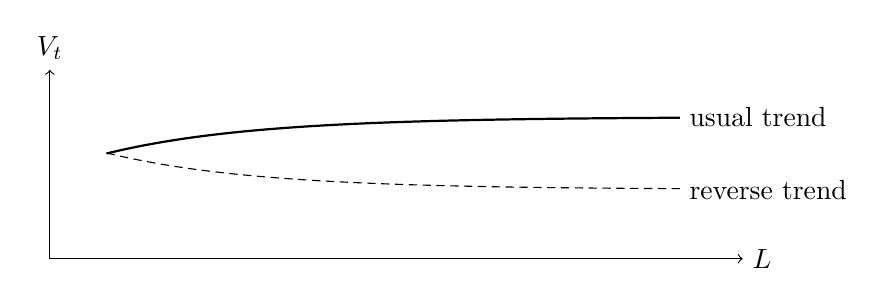
\begin{tikzpicture}[x=1.6cm,y=0.8cm]
 \draw[->] (0,0)--(5.5,0) node[right] {\(L\)};
 \draw[->] (0,0)--(0,3) node[above] {\(V_t\)};
 \draw[thick,domain=0.45:5,samples=60] plot (\x,{2.25-0.85*exp(-0.85*\x)});
 \draw[densely dashed,domain=0.45:5,samples=60] plot (\x,{1.1+0.85*exp(-0.85*\x)});
 \node[right] at (5,2.25) {usual trend};
 \node[right] at (5,1.1) {reverse trend};
\end{tikzpicture}
\end{latin}
\caption{طرح کیفی جهت تغییر آستانه با طول در دو رفتار توصیف‌شده در کتاب
و اسلاید ۲۰
\cite[بخش \secnum{۲.۴.۳.۳}]{weste}\cite{nonideal}.}
\label{fig:threshold-length-schematic}
\end{figure}

نام‌گذاری این قسمت از قرارداد کتاب برای وابستگی آستانه به طول پیروی
می‌کند. کتاب به کاربرد گسترده‌تر اصطلاح \lr{Short Channel Effect} برای
مجموعه اثرهای کانال کوتاه نیز اشاره می‌کند
\cite[پانوشت صفحه چاپی ۸۰]{weste}.

کتاب همچنین \lr{Narrow Channel Effect} را ذکر می‌کند که در آن آستانه
با عرض کانال تغییر می‌کند. اثر عرض معمولاً در مقایسه مورد بحث مرجع
کمتر است، زیرا حداقل عرض از حداقل طول بزرگ‌تر در نظر گرفته شده است
\cite[صفحه چاپی ۸۰]{weste}. مقدار و جهت وابستگی در یک افزاره مشخص به
ساختار و فرایند آن وابسته است.

با تغییر طول، ضریب \(\beta=\mu C_{\mathrm{ox}}W/L\) نیز تغییر می‌کند.
اگر مسئله، آستانه را تابع طول داده باشد، هم ضریب هندسی و هم
اضافه‌ولتاژ \(V_{GS}-V_t(L)\) باید به‌روزرسانی شوند.
در \lr{Channel Length Modulation} بخش \ref{sec:clm}، تغییر طول مؤثر
در اثر تغییر بایاس درین یک افزاره بررسی شد. در این قسمت، آستانه
افزاره‌ها با طول‌های مختلف مقایسه می‌شود.

در جدول \ref{tab:threshold-effects-summary} شرایط مقایسه سه اثر
گردآوری شده‌اند. علامت‌ها با قرارداد \lr{nMOS} بیان شده‌اند.
\begin{table}[!htbp]
\centering
\small
\caption{جهت تغییر آستانه در سه اثر این بخش، با ثابت بودن دیگر شرایط مقایسه.}
\label{tab:threshold-effects-summary}
\begin{tabularx}{\linewidth}{>{\raggedleft\arraybackslash}Xcc}
\toprule
اثر & متغیر مقایسه & نتیجه مدل\\
\midrule
\lr{Body Effect} & افزایش \(V_{SB}\) & افزایش \(V_t\)\\
\lr{DIBL} & افزایش \(V_{DS}\) & کاهش \(V_t\)\\
\lr{Short Channel Effect} معمول & کاهش \(L\) & کاهش \(V_t\)\\
رفتار \lr{Reverse Short Channel} & کاهش \(L\) & افزایش \(V_t\)\\
\bottomrule
\end{tabularx}
\end{table}
